\documentclass[aps,pra,notitlepage,amsmath,amssymb,letterpaper,12pt]{revtex4-1}
\usepackage{amsthm}
\usepackage{graphicx}
%  Above uses the Americal Physical Society template for Physical Review A
%  as a reasonable and fully-featured default template
 
%  Below define helpful commands to set up problem environments easily
\newenvironment{problem}[2][Problem]{\begin{trivlist}
\item[\hskip \labelsep {\bfseries #1}\hskip \labelsep {\bfseries #2.}]}{\end{trivlist}}
\newenvironment{solution}{\begin{proof}[Solution]}{\end{proof}}
 
% --------------------------------------------------------------
%                   Document Begins Here
% --------------------------------------------------------------

% In what follows, you can easily change text to see what happens to the document
% For example, replacing the text "Document X" inside the "\title{}" command will
% change the document title
 
\begin{document}
 
\title{CW 13--Analysis of CW 12}
\author{Abby Wheaton, Monica Hiemer, and Royal Cuevas}
\affiliation{PHYS 220, Schmid College of Science and Technology, Chapman University}
\date{\today}

\maketitle

\section{Objectives} % Specify main sections this way
In this Assignment we considered a ball of mass $m$ with horizontal coordinate $x$ rolling in a double-well potential $V(x) = x^4/4 - x^2/2$, also known as a sombrero. This potential produces a force $f_{\text{hat}}(x) = -V'(x) = -x^3 + x$ on the rolling ball. We suppose the ball also has slight friction, so experiences a drag force $f_{\text{drag}}(\dot{x}) = -\nu \dot{x}$. These forces would eventually make the ball come to a stop, so we also constered shaking the hat periodically with a driving force $f_{\text{drive}}(t) = F\cos(\omega t)$.
According to Newton's second law, the ball must satisfy the equation of motion: $$m\ddot{x} = f_{\text{hat}}(x) + f_{\text{drag}}(\dot{x}) + f_{\text{drive}}(t) = x - x^3 - \nu \dot{x} + F\cos(\omega t)$$ 
This system is known as a periodically driven nonlinear "Duffing oscillator," and can be split into a set of two coupled first-order ODEs:
$$\dot{x}(t) = y(t)$$
$$m\dot{y}(t) = -\nu y(t) + x(t) - x^3(t) + F\cos(\omega t)$$
In this assignment we used fourth order Runda Kutta for $m=1$, $\nu = 0.25$, and $\omega = 1$.


\section{Analysis of Solution}
Using the fourth order Runga Kutta method, we were able to plot the position of the rolling ball versus speed. We found that as the Force increases, the graph becomes more chaotic and it takes longer for the ball's speed and position to settle down. This observation is highlighted in the following two figures. The first has a Force value of 0.18. The second has a force value of 0.4.

\begin{figure}[h!] % h forces the figure to be placed here, in the text
  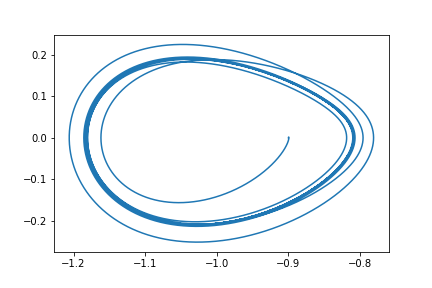
\includegraphics[width=0.8\textwidth]{sombrero2.png}  % if pdflatex is used, jpg, pdf, and png are permitted
  \caption{Graphical representation of the sombrero potential with a Force value of 0.18.}
  \label{fig:figlabel}
\end{figure}

\begin{figure}[h!] % h forces the figure to be placed here, in the text
  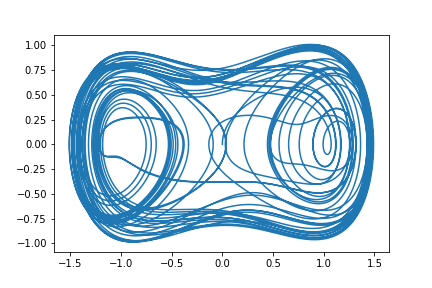
\includegraphics[width=0.8\textwidth]{sombrero3.png}  % if pdflatex is used, jpg, pdf, and png are permitted
  \caption{Graphical representation of the sombrero potential with a Force value of 0.4.}
  \label{fig:figlabel}
\end{figure}

\section{Conclusions}

To conclude, we have learned that fourth order Runga Kutta gives very accurate results in computing differential equations. The motion of the rolling ball starts out a little chaotic, but eventually settles down and becomes rather predictable. All in all, the previous assignment simply scratched the surface of the sombrero potential equation. It would be interesting to do more research into these equations.

 
\end{document}
